\documentclass[a4paper,10pt]{article}
\usepackage[scale=0.7,vmarginratio={1:2},heightrounded]{geometry}

\catcode`_=\active
\newcommand{_}{\ifmmode\expandafter\sbrm\else\string_\fi}
\newcommand{\sbrm}[1]{\sb{\mathrm{#1}}}

\usepackage{doc-setting}


\title{Arrangement of Polylines Traits Class - Upgrade}
\author{Dror Atariah}

\begin{document}
\maketitle

\begin{abstract}
  Outline the projects goals and progress.
\end{abstract}

\section{Introduction}
\label{sec:introduction}

The implementation of the computation of arrangement of polylines shipped with version 4.2 of \cgal proved to poses limitations.
For example, the only way it provides to construct a polyline is by giving a range of points as its input.
Another example would be that inspecting an existing polyline, in terms of iterating over its elements, is only possible by iterating over its \emph{vertices}.
These two main limitations, among others, turn it difficult to generalize the implementation --- for example when attempting to compute the arrangement of \emph{unbounded} polylines.
In addition, as the core of the code is several years old, it no longer meets the standards of \cgal.

Therefore, the goal of this project is, as a first step, to upgrade and update the code that deals with polylines in the Arrangement on Surface (AoS) package.
This upgrade lay the foundation for future generalization of the class.
In addition, by adopting better programming style we also manage to introduce an improvement of 5--7\% in the performance of the package.

\subsection{Notations Conventions}
\label{sec:notat-conv}

We use the following typesetting convention.
\begin{itemize}
\item \file{foo.bar} is a file name.
\item A concept is \concept{ConceptName} and its model is \model{Concept_name_model}.
\item \type{Some_type} will indicate a type and \functor{My_functor} will indicate a function class (a.k.a. functor).
\end{itemize}


\subsection{Definitions}
\label{sec:definitions}
%
Furthermore, we will use the following, more specific, conventions:
\begin{itemize}
%
\item \href{http://doc.cgal.org/4.2/CGAL.CGAL.2D-Arrangements/html/classCGAL_1_1Arr__polyline__traits__2.html}{\polytr} is the polyline traits class which currently models the following concepts:
  \begin{itemize}
  \item \concept{ArrangementTraits\_2}
  \item \concept{ArrangementLandmarkTraits\_2}
  \end{itemize}
  Its implementation can be found in \file{Arr\_polyline\_traits\_2.h}.
  This traits class has two nested types \poly and \xpoly which are the \type{Curve\_2} and \type{X\_monotone\_curve\_2} nested types of the traits class.
  These curves are the representations of piecewise linear (PL) curves and x-monotone PL curves respectively.
  \polytr, together with its nested curve types, is the component of the arrangement on surfaces package of \cgal which handles the construction and computations of arrangements of  sets of polylines.
  The actual implementations of \poly and \xpoly can be found in \file{Polyline\_2.h}.
%
\item The \concept{SegmentTraits} is the template parameter of the \polytr and it should be a model of \concept{ArrangementTraits\_2}.
  Currently there are two implementations of models of \concept{SegmentTraits}:
  \begin{itemize}
  \item \model{Arr\_segment\_traits\_2}
  \item \model{Arr\_non\_caching\_segment\_traits\_2}
  \end{itemize}
  When there is no place of confusion we shall refer to them as \segtr.
  In addition, \segtr models the concepts:
  \begin{itemize}
  \item \concept{ArrangementTraits\_2}
  \item \concept{ArrangementLandmarkTraits\_2}
  \item \concept{ArrangementDirectionalXMonotoneTraits\_2}
  \end{itemize}
  For example, \model{Arr_segment_traits_2} is implemented in \file{Arr\_segment\_traits\_2.h}.
  Let \seg be the \type{Curve\_2} and \type{X\_monotone\_curve\_2} nested types that are nested in \segtr.
\end{itemize}

\section{Implementation of \poly and \xpoly}
\label{sec:implementation-poly}

The implementations of \poly and \xpoly are the building blocks of the polyline traits class and the way we could compute arrangement of polylines.
The existing implementation of the types is rather old  and no longer meets the standards of \cgal.
Furthermore, as we discuss later, the implementation is restrictive and cannot serve in an attempt to generalize the package to support \emph{unbounded polylines}.
Therefore, this implementation had to be revised and we discuss this revision in this section.

\paragraph{Degenerated polylines.}
\label{sec:degen-polyl-construction}

The \segtr does not allow the construction of degenerated polylines.
In turn, we impose a similar constrain on the construction of \poly and \xpoly, namely we exclude the construction of degenerated polylines.
That is we do not treat polylines which contains degenerated segments (i.e. segments of length zero) and isolated points.

\paragraph{Well oriented polylines.}
\label{sec:well-orient-polyl}

From a strictly mathematical point of view, polylines do not induce any notion of orientation.
Here orientation is in the sense of source or start of a polyline and its target or end.
The only restriction is that the constituting segments will concatenate properly and form a PL curve.
Similarly, the segments, again from a mathematical point of view, may not be directed.
However, the both implementations of models of \concept{SegmentTraits} model the concept \concept{ArrangementDirectionalXMonotoneTraits_2}.
In other words they provide the notion of both \emph{source} and \emph{target}.
The source and target of a segment can be determined using the functors
\begin{itemize}
\item \functor{Compare\_endpoints\_xy\_2}
\item \functor{Construct\_opposite\_2}
\end{itemize}
which are provided by \concept{ArrangementDirectionalXMonotoneTraits_2} together with the functors
\begin{itemize}
\item \functor{Construct\_min\_vertex\_2}
\item \functor{Construct\_max\_vertex\_2}
\end{itemize}
which are defined in the concept \concept{ArrangementTraits_2}.
Furthermore, two access function \code{source()} and \code{target()} are provided by \segtr.
Note that these functions are \emph{not} required by the concepts which \segtr models.
Nevertheless, current implementation of \poly and \xpoly used these function extensively.
Obviously this is bad programming style.

In order to keep the efficiency benefits of the usage of \code{source()} and \code{target()} on one hand and consistency with the documentation on the other, we add a requirement that \segtr should be model of the \concept{ArrangementDirectionalXMonotoneTraits\_2}.
Note that this assumption implies only a conceptual restriction, since in practice the available implementations that can be used model this concept anyway.
Once \segtr models this concept we can remove all occurrences of \code{source()} and \code{target()}.
In this we assert that \polytr itself will be a model of this concept as well.
As a result, we can also provide the following invariant: \textbf{\poly and \xpoly will be \emph{well oriented}.}\marginpar{\footnotesize{\emph{well oriented}}}
That is, the \emph{source} of the \(n\)-th \seg should be the \emph{target} of the \((n-1)\)-th \seg.
In particular the polyline:
\begin{center}
  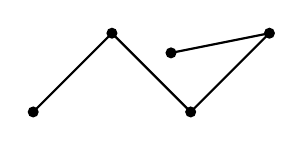
\begin{tikzpicture}
    \begin{scope}[thick]
      \draw (-2,0) coordinate (a1) -- (-1,1) coordinate (a2);
      \draw (0,0) coordinate (a3) -- (a2);
      \draw (1,1) coordinate (a4) -- (a3);
      \draw (a4) -- (-0.25,0.75) coordinate (a5);
      \foreach \i in {1,2,3,4,5}
      \fill (a\i) circle (2pt);
    \end{scope}
  \end{tikzpicture}
\end{center}
can now be represented as one and only one of the following:
\begin{center}
  \begin{tikzpicture}
    \begin{scope}[thick,decoration={%
        markings,
        mark=at position 0.5 with {\arrow{>}}%
      }]
      \coordinate (a1) at (-2,0);
      \coordinate (a2) at (-1,1);
      \coordinate (a3) at (0,0);
      \coordinate (a4) at (1,1);
      \coordinate (a5) at (-0.25,0.75);
      \draw[postaction={decorate}] (a1) -- (a2);
      \draw[postaction={decorate}] (a2) -- (a3);
      \draw[postaction={decorate}] (a3) -- (a4);
      \draw[postaction={decorate}] (a4) -- (a5);
      \foreach \i in {1,2,3,4,5}
      \fill (a\i) circle (2pt);
    \end{scope}
    %
    \begin{scope}[xshift=4cm,thick,decoration={%
        markings,
        mark=at position 0.5 with {\arrow{>}}%
      }]
      \coordinate (a1) at (-2,0);
      \coordinate (a2) at (-1,1);
      \coordinate (a3) at (0,0);
      \coordinate (a4) at (1,1);
      \coordinate (a5) at (-0.25,0.75);
      \draw[postaction={decorate}] (a2) -- (a1);
      \draw[postaction={decorate}] (a3) -- (a2);
      \draw[postaction={decorate}] (a4) -- (a3);
      \draw[postaction={decorate}] (a5) -- (a4);
      \foreach \i in {1,2,3,4,5}
      \fill (a\i) circle (2pt);
    \end{scope}
  \end{tikzpicture}
\end{center}

\paragraph{Direction invariant of \(x\)-monotone polylines.}
\label{sec:direct-invar-x-mono-poly}

An \xpoly is x-monotone regardless of its representation.
X-monotonicity is a geometrical property of the polyline, and it is not by its internal representation.
Currently, an \xpoly maintains a \emph{direction invariant}\marginpar{\footnotesize{\emph{direction invariant}}} that it is oriented \emph{left-to-right}.
That is, its vertices should be given in an increasing lexicographic order.
However, in general an \xpoly should merely be x-monotone, and its vertices (or segments) may be oriented from left-to-right \emph{or} from right-to-left.
In this project we lifted this restriction and the new implementation allows the construction of \xpoly's which are oriented either left-to-right \emph{or} right-to-left.

\paragraph{Accessing the traits class from nested types.}
\label{sec:access-traits-class-from-nested-types}

\cgal's style discourages the usage of functors from traits classes inside nested types.
The current implementation violated this style.
Therefore all cases where functors of either \polytr or \segtr were used inside \poly and \xpoly were removed.
This includes removing code which was in \code{CGAL_precondition}.

\paragraph{Name spaces.}
\label{sec:name-spaces-poly+xpoly}

The implementation of \poly and \xpoly was moved into its own namespace, namely \code{POLYLINE}.\todo{What should I add here? Is it enough?}


\paragraph{Construction and Iteration.}
\label{sec:constr+iter-poly}

The current implementation of \poly and \xpoly emph{relays on their vertices} and it is only possible to construct the from a given range of \emph{points}.
Furthermore, given either a \poly or \xpoly, it is only possible to iterate over its vertices.
There is no way to iterate over the segments that constitute the polyline.
This design limits the possibilities of extending the traits class, for example to enable the handling of unbounded polylines.

\subparagraph{Construction.}
In order to enable construction of unbounded polylines, we have to add the possibility of construction from ranges of \seg's.
Ultimately, there will be \emph{only} one constructor of either \poly's or \xpoly's.
This construction will construct the polyline \emph{only} from ranges of \seg's.
For the sake of backwards compatibility, the current constructor, namely the one from a range of points, will be kept as deprecated\footnote{In the next version it will be removed completely.}.

The user should be encouraged to use the construction functors from \polytr (see \cref{sec:constr-funct-polytr}) and not the direct constructor of the class.
The functors provide the construction from two points, one segment, range of points and range of segments.

\subparagraph{Iteration.}
As we pointed out, iteration over the vertices of the polyline is restrictive.
We thus replace the iterators over the vertices which are currently defined for \poly and \xpoly with iterators over the segments of \poly and \xpoly respectively.
The iterators over the segments are obtained directly from the container of the \seg's.
Note that due to this change all the occurrences of iterators over the points of either a \poly or an \xpoly in \polytr have to be replaced with the iterators over their respective segments.

\paragraph{Augmenting a polyline}
\label{sec:augmenting-poly}

Currently, a polyline can be augmented using a \emph{push-back} function.
This function works as follows:
\begin{enumerate}
\item Gets a vertex as its input.
\item Obtains the last vertex of the polyline using \code{target()} function.
\item Generates a new \seg and pushes it to the range of segments representing the \poly.
\end{enumerate}
As we already mentioned, using a function like \code{target()} has to be avoided.
Furthermore, in order to maintain the well-orientedness of the polylines \segtr has to be used; again this is not desired
Augmenting an existing polyline will be treated, from now on, using the functor \functor{Push_back_2} (See \cref{sec:augmenting-poly-in-polytr}).

\section{Changes and updates of  \polytr}
\label{sec:impl-polytr}

Ultimately, the \polytr should be in charge of all the operations which deal with \poly's and \xpoly's.
To that end, the traits class should provide functors which construct, augment, split etc. polylines.

\subsection{Construction Functors}
\label{sec:constr-funct-polytr}

As we leave only one constructor (which handles a range of \seg's) in the class of \poly and \xpoly we have to provide other needed construction methods in the traits class, namely in \polytr.
To that end we provide two functors \functor{Construct_curve_2} and \functor{Construct_x_monotone_curve_2} which returns either a \poly or \xpoly object respectively.
The \code{operator()} of these functors is overloaded so it can treat various types of inputs.
In particular we provide the following overloads in the \functor{Construct_curve_2}
\begin{pyglist}[language=c++]
  Curve_2 operator()(const Point_2& p, const Point_2& q) const
  Curve_2 operator()(const Segment_2& seg) const
  Curve_2 operator()(ForwardIterator begin, ForwardIterator end) const
\end{pyglist}
\noindent
The last functor dispatches the given range to the corresponding implementation depending on the \emph{type} of the elements of the given range.
Similar functors are provided for the construction of \xpoly.
All validity tests of the input should be done in \code{CGAL\_precondition} blocks.

\subsection{Augmenting a \poly or \xpoly}
\label{sec:augmenting-poly-in-polytr}

We added the functor \functor{Push_back_2} which augment either an existing \poly or \xpoly.
Note that ideally, the user would not have to use augment an \xpoly manually.
The functor is able to append either vertices or segments to an \emph{existing} (\(x\)-monotone) polyline.
Note that once the polyline will be unbounded augmentation will not be always possible.

\subsection{Output of \functor{Intersect\_2}}
\label{sec:outp-funct-intersect-2}

In the concept \concept{ArrTraits::Intersect\_2} it is defined that the output iterator should contain the elements in an ascending \(xy\)-lexicographic order.
Thus, obviously, the implementation of \functor{Intersect\_2} had to be updated one the left-to-right invariant was lifted.

\subsection{Location Functions}
\label{sec:location-functions-polytr}

Due to the lifting of the left-to-right invariant of the x-monotone polylines, the functions \code{locate()} and \code{locate\_side()} had to be corrected.
During the correction a mistake in the original implementation was found.
Consider the following simple example.
Set \(p_0 = (-1,0), p_1 = (0,0)\) and \(p_2 = (1,0)\) and let \(c\) be the \(x\)-monotone polyline which connects them.
Next, let \(q = (0,1)\) be the query point.
\begin{center}
  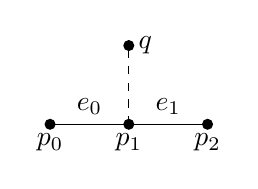
\begin{tikzpicture}
    \coordinate (p0) at (-1,0);
    \coordinate (p1) at (0,0);
    \coordinate(p2) at (1,0);
    \coordinate(q) at (0,1);
    \draw (p0) --node[above]{$e_0$} (p1) --node[above]{$e_1$} (p2);
    \foreach \i in {0,1,2}
    \fill (p\i)node[below]{$p_{\i}$} circle (2pt);
    \fill (q)node[right]{$q$} circle (2pt);
    \draw[dashed] (p1) -- (q);
  \end{tikzpicture}
\end{center}
In the original implementation \code{_locate(seg_tr,c,q)} would return the index \(i=0\).
But in this case neither of the tests
\begin{pyglist}
  if (equal(segment_traits_2()->construct_min_vertex_2_object()(cv[i]), q))
  if (equal(segment_traits_2()->construct_max_vertex_2_object()(cv[i]), q))
\end{pyglist}
\noindent would yield \emph{TRUE} and thus \code{_locate_side(seg_tr,c,q,ture)} would return \(i=0\), while it \emph{should} yield \(i=1\).

\subsection{Changes Derived from \poly}
\label{sec:changes-derived-from-polytr}

As a result of the changes in \poly and \xpoly (cf. \cref{sec:implementation-poly}), updates and modifications are needed also in \polytr.
In particular the lifting of the left-to-right direction invariant of the \(x\)-monotone polylines forced changes in almost \emph{all} functors of \polytr.
Most significant functors which were influenced by this change were:
\begin{itemize}
\item \functor{Make_x_monotone_2}
\item \functor{Intersect_2}
\item \functor{Merge_2}
\item \functor{Split_2}
\end{itemize}

\section{Testing the Code}
\label{sec:testing-code}

The original tests which were carried out were limited and naturally did not consider the cases of \(x\)-monotone polylines which are oriented right-to-left.
Thus, in order to verify that the upgraded implementation is correct, we extended the tests so they cover the cases of inverse \(x\)-monotone polylines.

\paragraph{\functor{Intersect_2}:}
\label{sec:testing-intersect_2}

\cref{fig:test-cases-of-intersect_2} illustrates all the \xpoly's that we considered in out testings.
Note that we considered all the possible pairs of \xpoly's that arise from the family of \(x\)-monotone polylines that we consider in the image.

\begin{figure}
  \centering
  \includegraphics[width=\linewidth]{./figures/intersect}
  \caption{The \xpoly's used in testing \functor{Intersect_2}}
  \label{fig:test-cases-of-intersect_2}
\end{figure}

Interesting cases:
\begin{itemize}
\item The intersection of the pair of \xpoly's \(\{12,34\}\) and \(\{12,13\}\).
It finds the intersection point, namely \((1,1)\) but with multiplicity \(0\)\todo{Shouldn't it be multiplicity \(1\)?}.
For example, the \xpoly number 34, passes through the vertex \((1,1)\) of the \xpoly number 12.
Similar issue arises for example with the pair \(\{13,34\}\) or with the pair \(\{15,35\}\).
\end{itemize}

\section{Benchmark}
\label{sec:benchmark}

Once we finished testing the code we benchmarked the code in order to verify that the changes did not impair the performances.
Indeed, the usage of advanced coding resulted in an improvement of \(4.8\%\) in average.
For the benchmark we used the code which can be found in \file{bench_random_arr_polylines.cpp} in \file{Arrangement_on_surface_2/benchmark/Arrangement_on_surface_2}.
Note that this code uses the \emph{deprecated} construction of polylines -- we did it in order to run the same benchmark both on the original implementation and on our improvement.
\cref{tab:benchmark-results} in \cref{sec:summ-benchm-tests} summarizes the results of the benchmarks.


\section{Future Work}
\label{sec:future-work}

\begin{itemize}
\item Re-implement \code{locate()} so it will return a \emph{pointer} rather then an index to the containing segment.
\item Fix \functor{Make_x_monotone_2} so it will not depend on the input's order.
Consider the following example.
Let \(T\) be the triangle defined by the vertices \(p_1 = (0,2), p_2 = (-1,-1)\) and \(p_3 = (1,-1)\).
From a strictly mathematical point of view the \(T\) can be treated as a polyline, and in turn the induced arrangement would consist of \emph{one} vertex, one edge (the triangle \(T\) itself) and \emph{two faces}.
Since the implementation of the arrangement package depends on the notion of \(x\)-monotone curves, we cannot avoid having \emph{two} vertices and \emph{two} edges in the resulting arrangement.
However, depending on the order in which the points are given the current implementation can yield different results.
The triangle defined by \(\overline{p_2 p_1 p_3 p_2}\) yields \((2,2,2)\) as its \(f\)-vector, whereas \(\overline{p_1 p_2 p_3 p_1}\) yields the \(f\)-vector \((3,3,2)\).
Note that the number of face is correct, but the other elements of the vector are not stable.
\item Accessing the segments of a polyline.
  Currently accessing a segment of either a \poly or \xpoly is done using the \code{operator[]}.
  Replace this accessing method with iterators/handles.
\end{itemize}

\appendix

\section{Summary of benchmark tests}
\label{sec:summ-benchm-tests}

\begin{landscape}
  \begin{table}
    \centering
    \begin{tabular}{rrrrrrrrr}
      \hline
      Seed & N & V & E & F & Timer (B) & Timer (M) & \%  & Mean \% \\
      \hline
      \hline
      1368346973 & 10 & 10 & 12 & 4 & 0.000768 & 0.000712 & -7.8651685 &  \\
      \hline
      1368346990 & 10 & 7 & 9 & 4 & 0.000673 & 0.000608 & -10.690789 &  \\
      \hline
      1368347002 & 10 & 10 & 13 & 5 & 0.000716 & 0.000674 & -6.2314540 & -8.2624705 \\
      \hline
      1368347036 & 50 & 326 & 615 & 291 & 0.017041 & 0.017389 & 2.0012652 &  \\
      \hline
      1368347050 & 50 & 259 & 485 & 228 & 0.013991 & 0.01423 & 1.6795502 &  \\
      \hline
      1368347062 & 50 & 254 & 471 & 219 & 0.013594 & 0.014035 & 3.1421446 & 2.27432 \\
      \hline
      1368347141 & 500 & 29357 & 58378 & 29023 & 1.50945 & 1.65587 & 8.8424816 &  \\
      \hline
      1368347165 & 500 & 26395 & 52464 & 26071 & 1.36537 & 1.44331 & 5.4000873 &  \\
      \hline
      1368347184 & 500 & 27592 & 54847 & 27257 & 1.4248 & 1.50637 & 5.4150043 & 6.5525244 \\
      \hline
      1368347214 & 1000 & 117252 & 233848 & 116598 & 6.13624 & 6.39283 & 4.0137154 &  \\
      \hline
      1368347267 & 1000 & 115255 & 229844 & 114591 & 6.05129 & 6.32789 & 4.3711253 &  \\
      \hline
      1368347320 & 1000 & 122911 & 245155 & 122246 & 6.41939 & 6.78416 & 5.3767895 & 4.5872101 \\
      \hline
      1371453603 & 2000 & 453785 & 906218 & 452435 & 24.2019 & 25.3598 & 4.5658877 &  \\
      \hline
      1371453661 & 2000 & 472734 & 944122 & 471390 & 25.1665 & 26.2028 & 3.9549208 &  \\
      \hline
      1371453708 & 2000 & 450377 & 899397 & 449022 & 23.8502 & 24.9693 & 4.4819038 & 4.3342374 \\
      \hline
      1371453752 & 2500 & 710089 & 1418556 & 708469 & 37.8684 & 39.9537 & 5.2192913 &  \\
      \hline
      1371453814 & 2500 & 739811 & 1477940 & 738131 & 39.4883 & 41.7421 & 5.3993450 &  \\
      \hline
      1371453926 & 2500 & 730482 & 1459272 & 728792 & 40.0593 & 40.8858 & 2.0214842 & 4.2133735 \\
      \hline
      1371453996 & 3000 & 1041705 & 2081422 & 1039719 & 56.5583 & 60.2639 & 6.1489548 &  \\
      \hline
      1371454074 & 3000 & 1024104 & 2046202 & 1022100 & 55.2771 & 61.2115 & 9.6949103 &  \\
      \hline
      1371454144 & 3000 & 1011434 & 2020912 & 1009480 & 54.5034 & 57.0535 & 4.4696644 & 6.7711765 \\
      \hline
    \end{tabular}
    \caption{Benchmark results}
    \label{tab:benchmark-results}
  \end{table}
\end{landscape}


\end{document}

%%% Local Variables:
%%% mode: latex
%%% TeX-master: t
%%% End:
